\documentclass{article}   

\usepackage[lighttt]{lmodern}
\usepackage{url}    
\usepackage{attachfile2}   
\usepackage{natbib}
\usepackage{graphicx}
\usepackage{placeins}
\usepackage{tabularx,ragged2e,booktabs,caption}
\usepackage{pdflscape}
\usepackage{tocbibind}
\usepackage{tocloft}

% \usepackage[none]{hyphenat}


 


\renewcommand{\abstractname}{\vspace{-\baselineskip}}
\DeclareTextFontCommand{\codefont}{\ttfamily \bfseries}
\setcounter{secnumdepth}{-2}

\begin{document}

\title{Nowcasting for BC Hydro: EmWxNet data assimilation project}
\author{Nadya Moisseeva}
\date{April 2015}    % type date between braces

\maketitle
% \begin{center}
% \begin{figure}[h]
% 	\includegraphics[height=14cm]{../logo.pdf}
% \end{figure}
% \end{center}

\tableofcontents

\newpage
\section{Data and coverage}
\subsection{WRF forecast field data}
Temperature (2 meters), wind and precipitation data are obtained from UBC WRF-GFS runs for a 4km domain. Points falling within the selected -129W-120W longitude and 48N-52M latitude bounded area are extracted. Figure \ref{T2raw} shows the obtained data overlayed on a standard grid for the temperature field. 
\begin{figure}
\makebox[\textwidth][c]{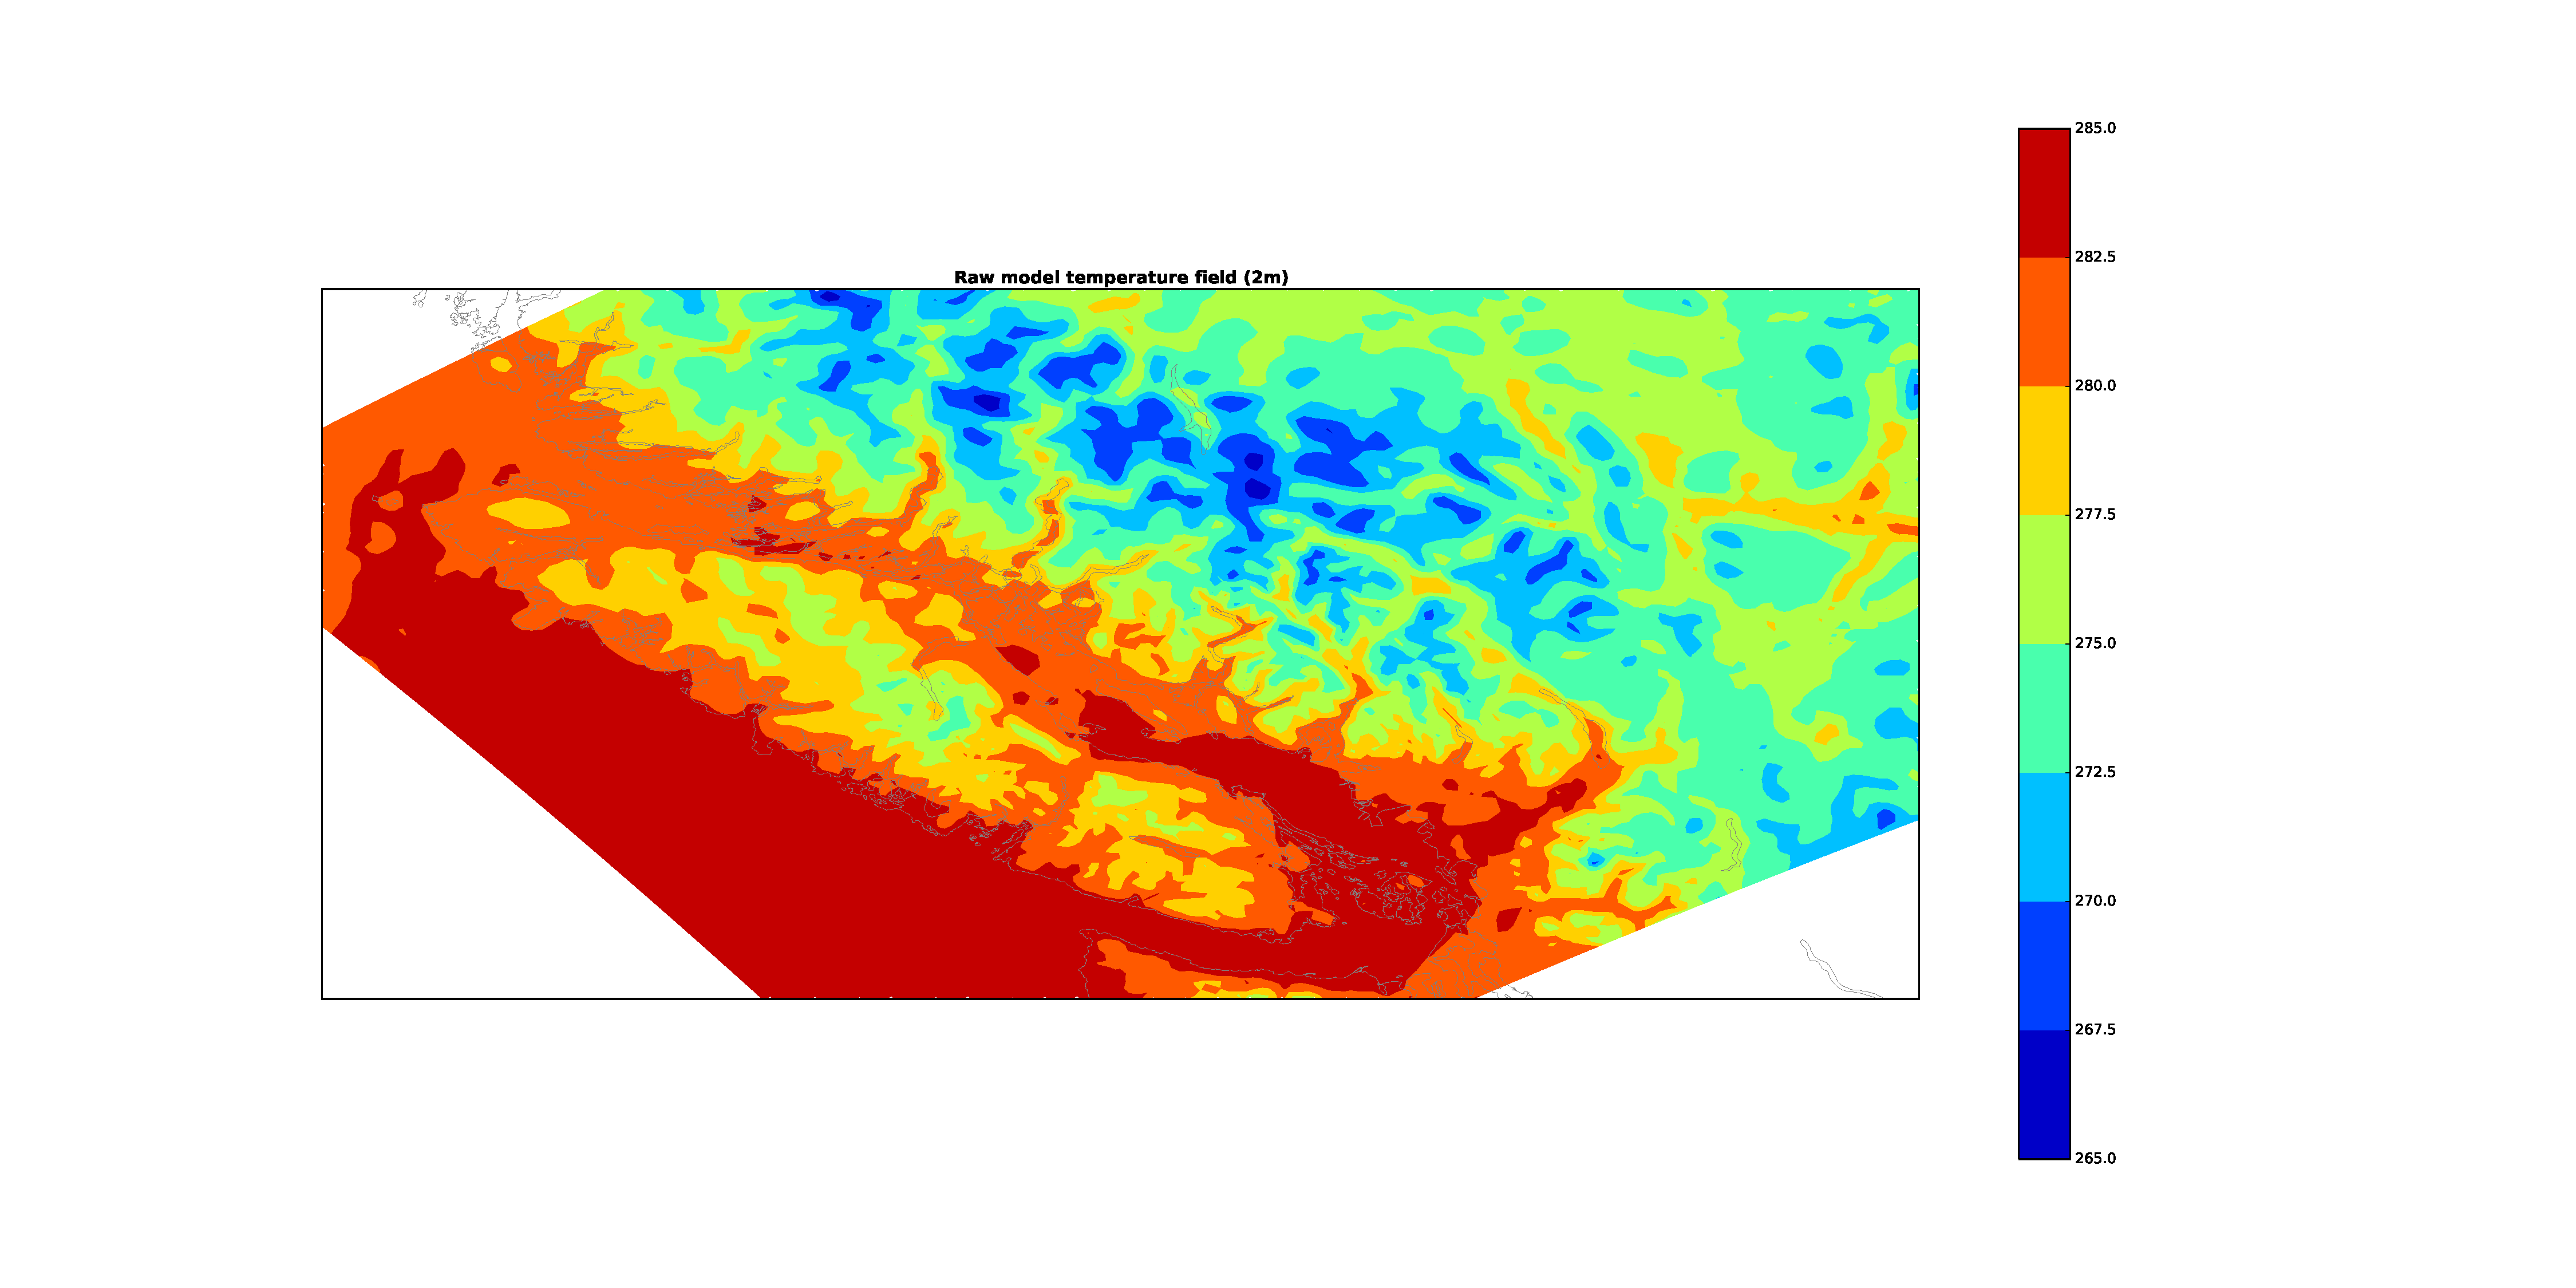
\includegraphics[width=2\textwidth]{../temp_raw.pdf}}
\caption{Raw model (forecast) data on a strandard lon-lat grid for Feb 19, 2015 at 1800.}\label{T2raw}
\end{figure}

\subsection{EmWxNet data}
A C routine was developed based on the EmWxNet API system, to extract select stations falling within the desired domain. Station meta as well as weather data are subsequntly downloaded and saved. A total of over 500 stations fit the criteria, however apprixmately 300 stations actually contain useful data. The spatial distribution of stations is shown in Figure \ref{Domain}. Note that points falling within the boundaries of US are excluded, due to lack of elevation data for the area. 

\subsection{DEM data}
Surface elevation data was obtained from Natural Resources Canada [available at: \url{http://geogratis.gc.ca/site/eng/extraction?layers=cdsm&bbox=-139.5,48,-113.5,60}]. CDEM dataset was extracted for the above-mentioned domain at 12 arcsecond ($\approx$330m) resolution in GeoTIFF format (shown in Figure \ref{Domain})
\begin{figure}
\makebox[\textwidth][c]{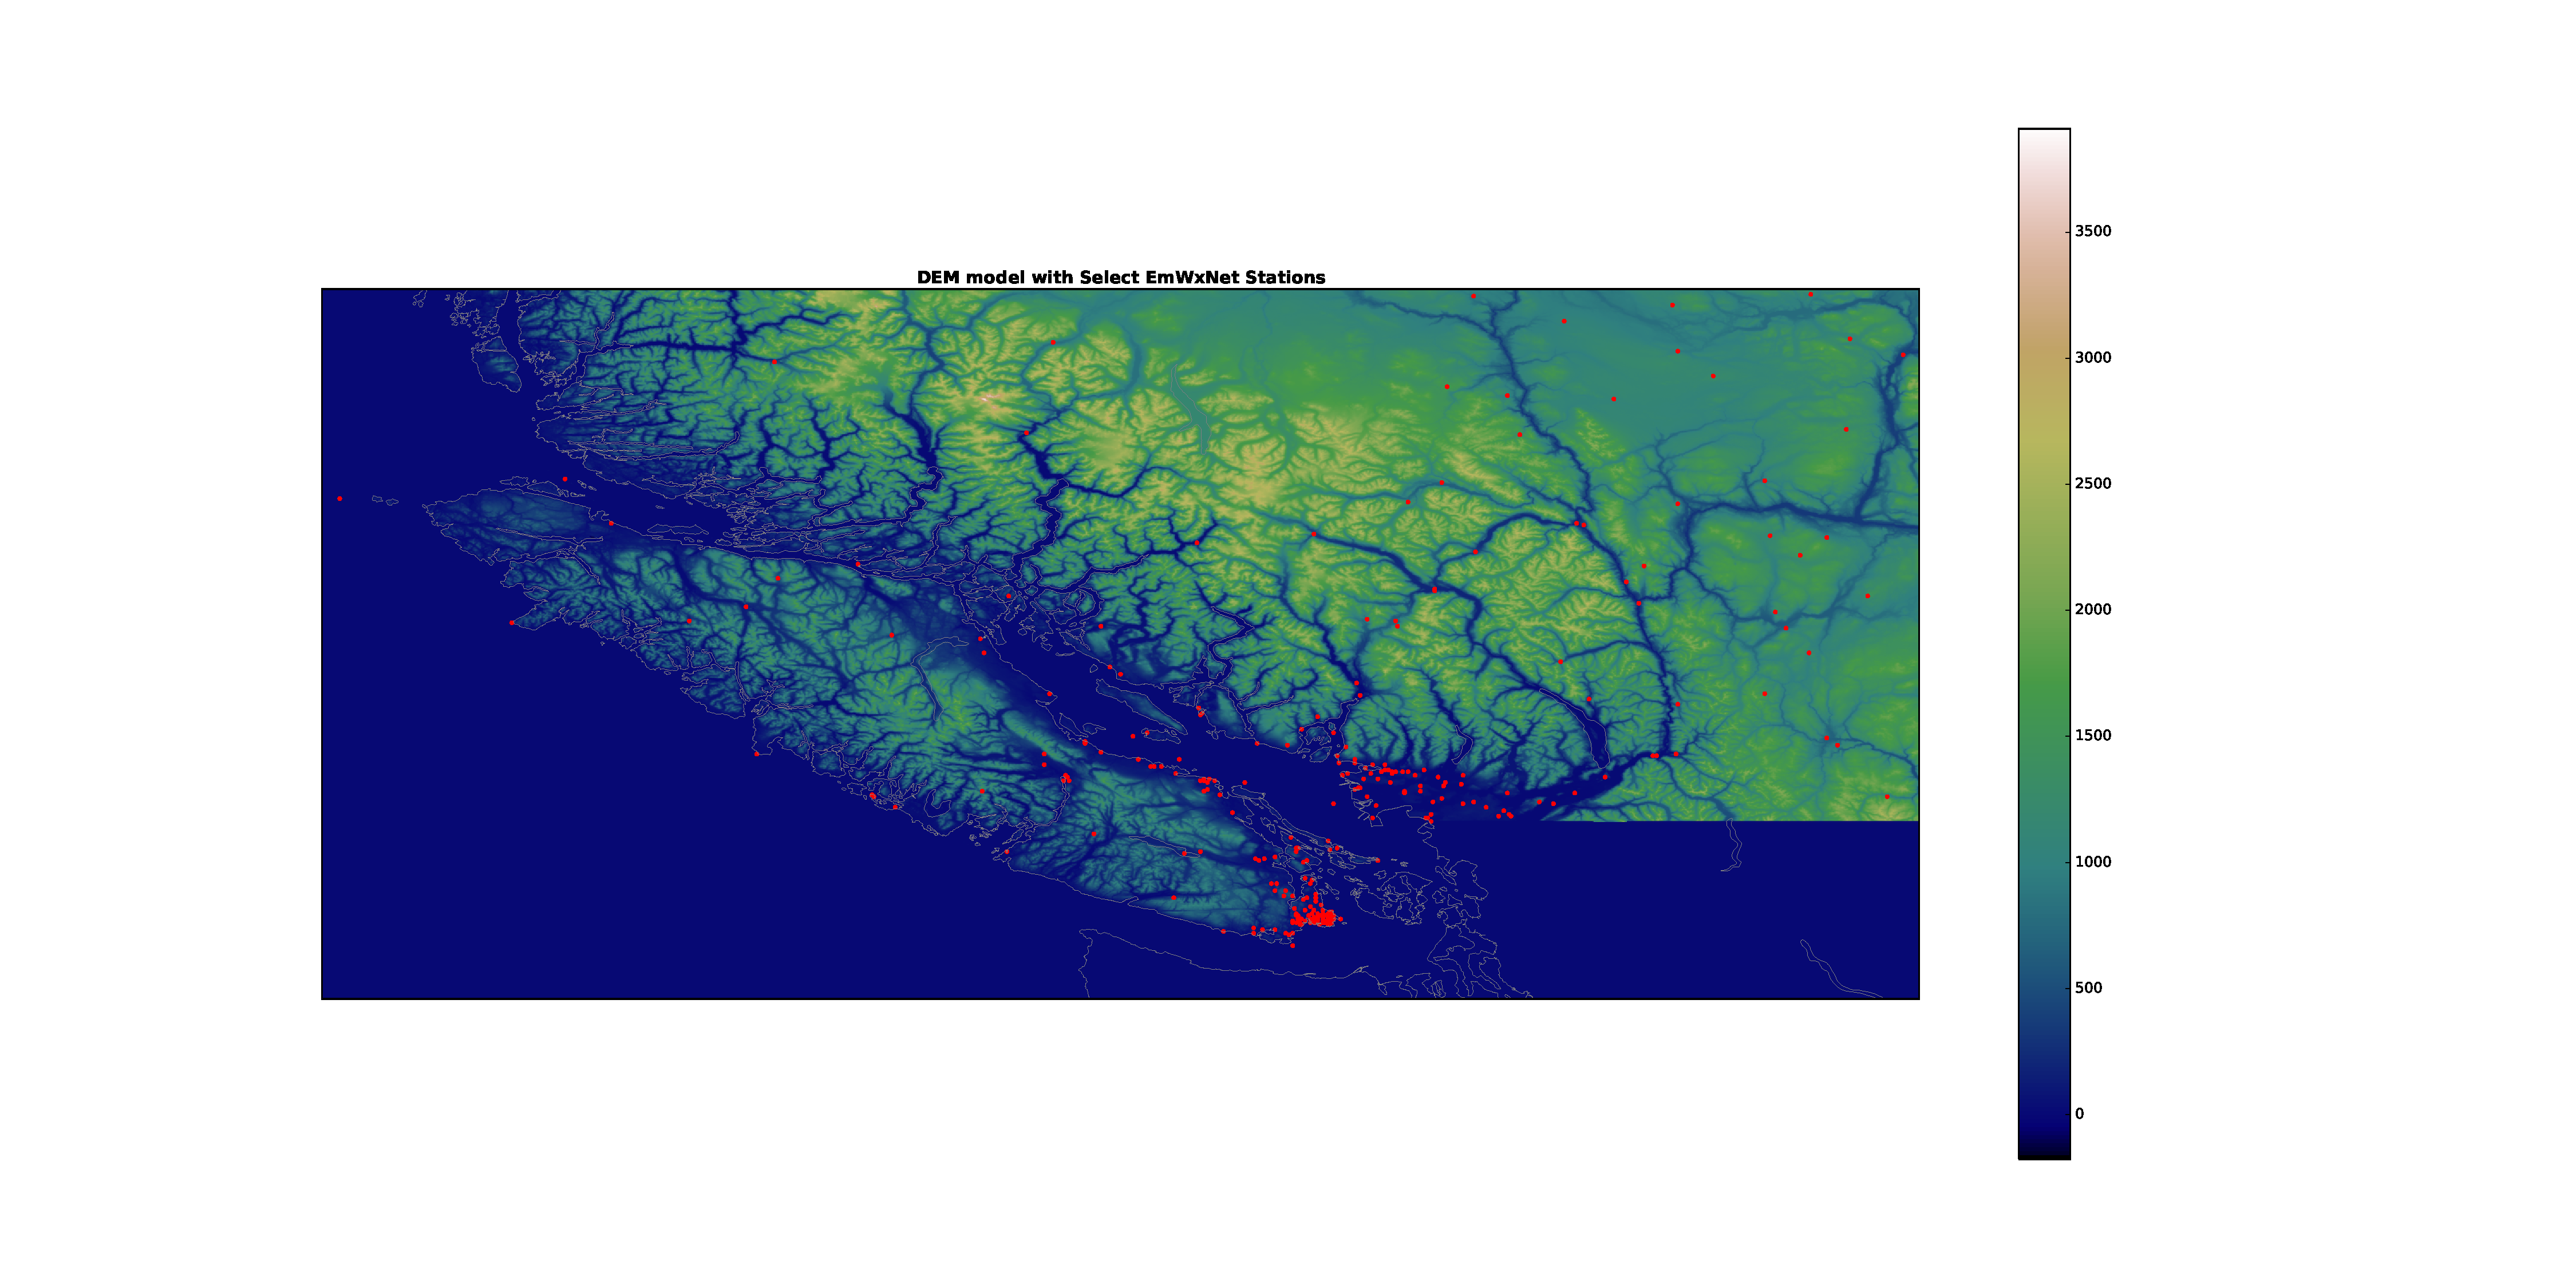
\includegraphics[width=2\textwidth]{../DEM_obs_12arcsec.pdf}}
\caption{EmWxNet station locations shown in red, over 12 arcsecond DEM grid.}\label{Domain}
\end{figure}

The remainder of data shown in the figures (eg coastlines, boundaries) are provided by Python standard Matplotlib.basemap package. 

\section{Temperature Downcaling}
\begin{figure}
\makebox[\textwidth][c]{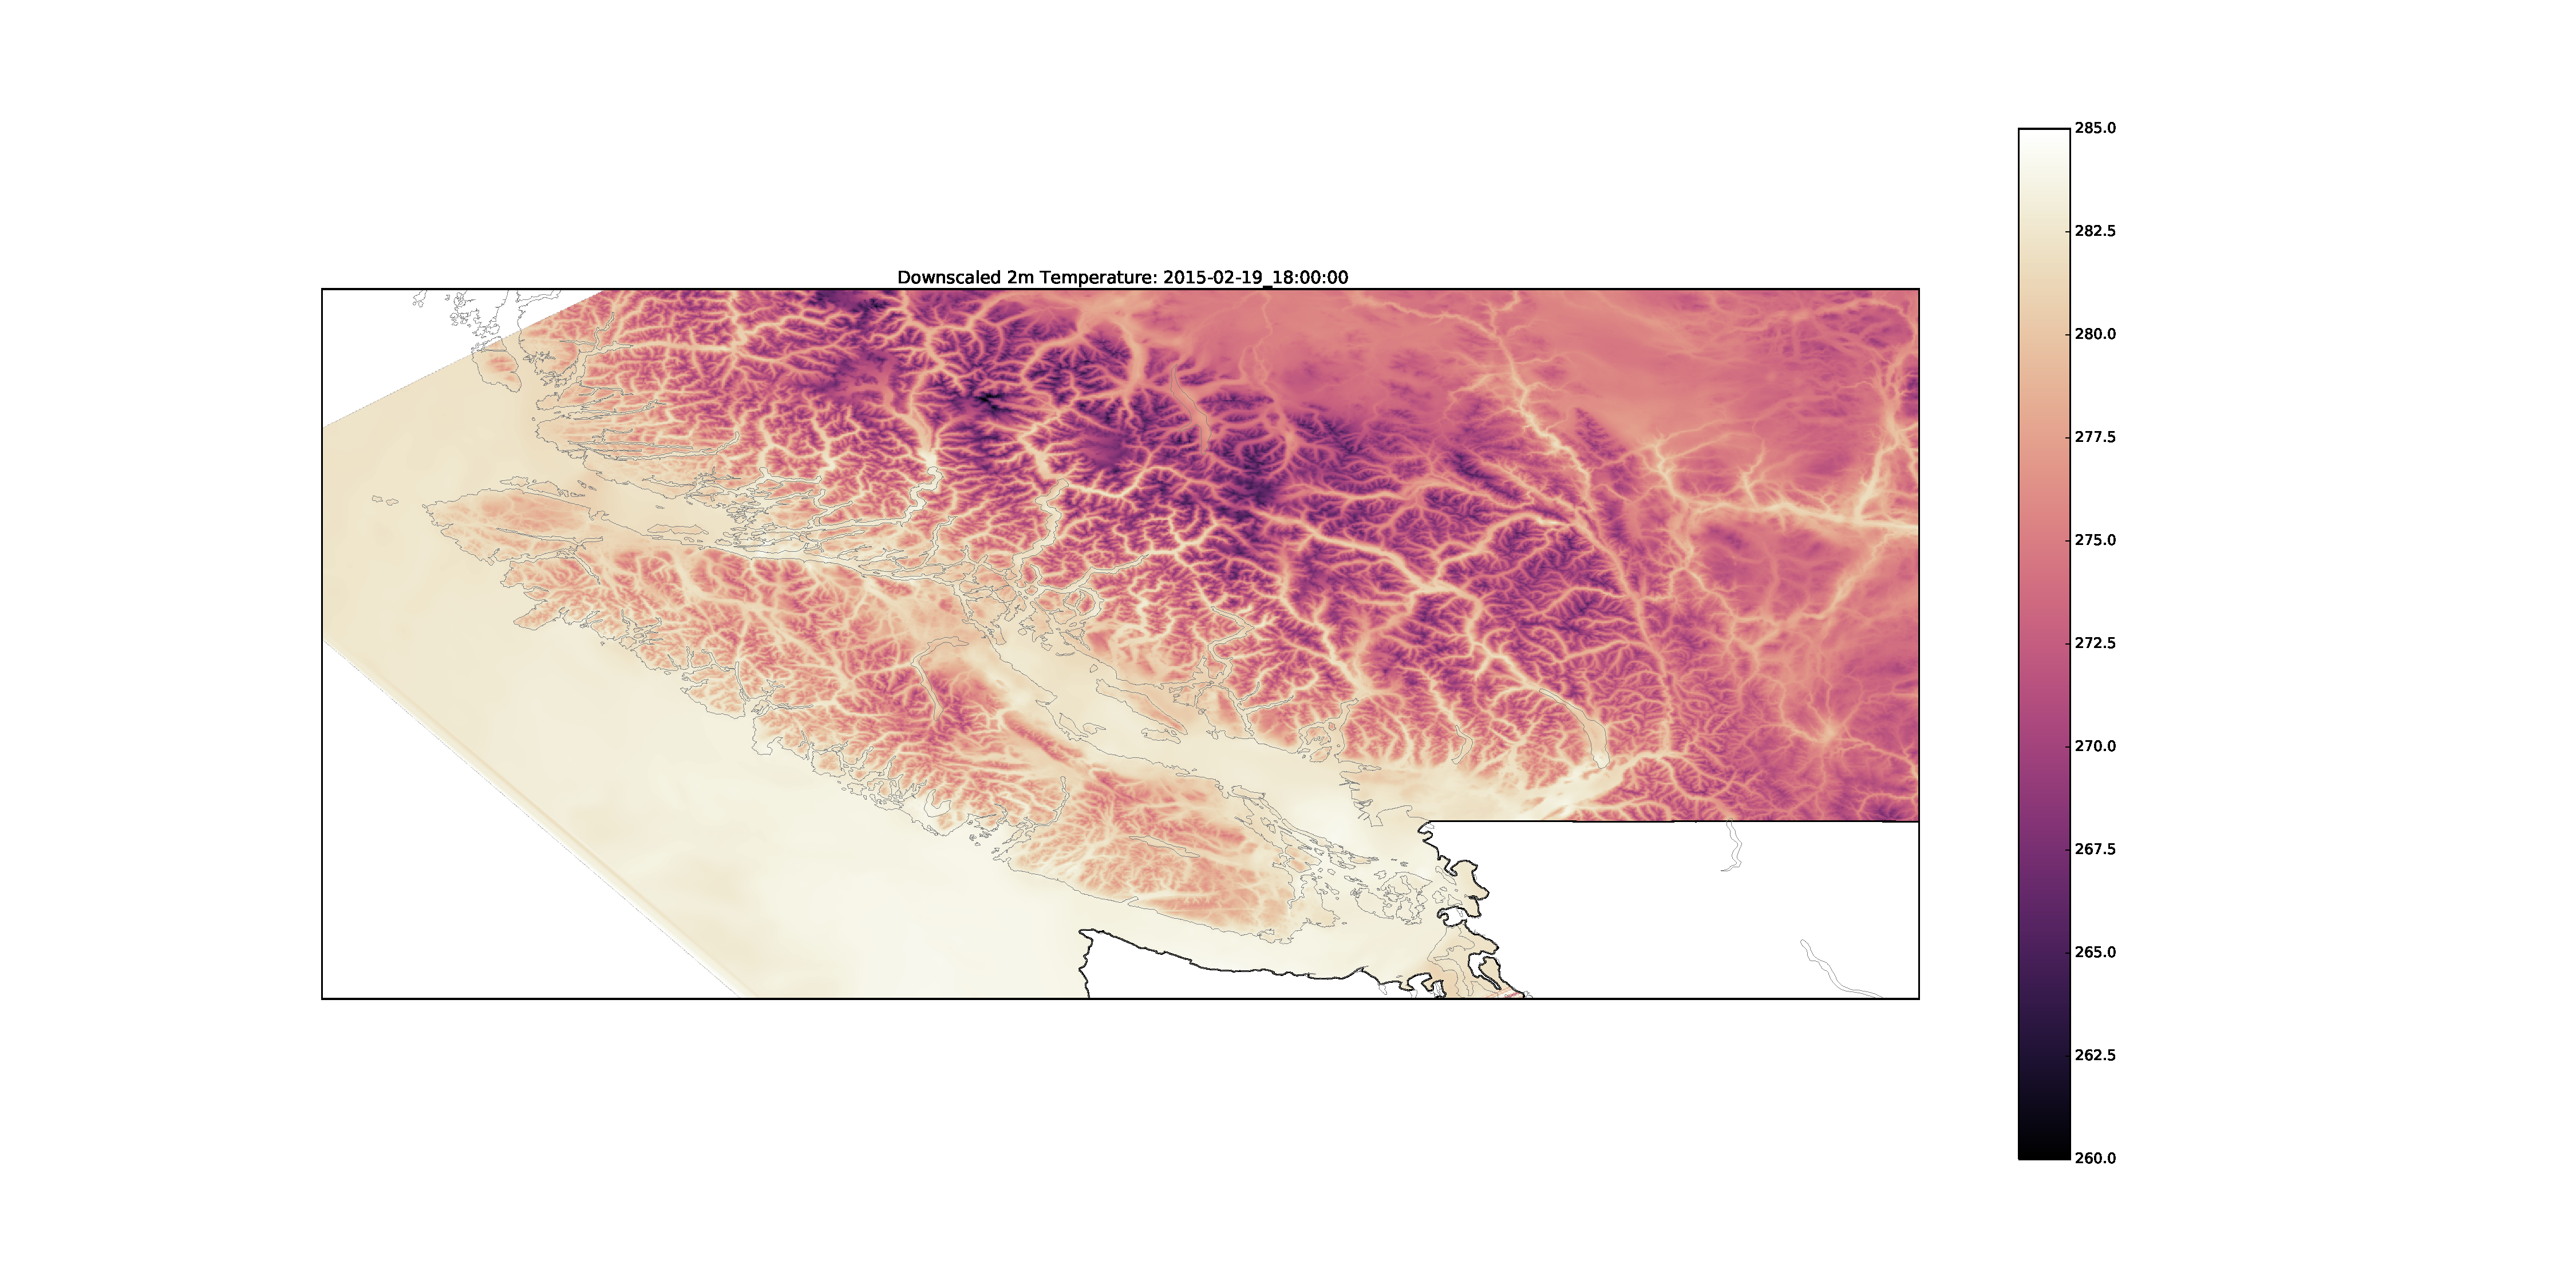
\includegraphics[width=2\textwidth]{../DownscaledT2.pdf}}
\caption{Downscaled temperature using constant lapse rate.}\label{demT2}
\end{figure}
\begin{figure}
\makebox[\textwidth][c]{\includegraphics[width=1.6\textwidth]{../VerificatinPlotT2.pdf}}
\caption{Regression analysis of raw forecast and downscaled temperature data.}\label{scatterT2}
\end{figure}


% \bibliographystyle{agu08}
% \bibliography{summary}

\end{document}

